\documentclass[UTF8]{ctexart}

\usepackage{subfiles}  

%下面的语句, 引入你的头部设置文件
\usepackage{C:/phpStorm_proj/02_myself_ID_EGO/+100_latex_all_math_sel/myPreamble} 
%必须是绝对路径,才能让各个tex在单独编译时使用到

\title{文件名}


%---------------------------------


\begin{document}
	\tableofcontents % 生成目录
	\date{} % 若不写这句, 则默认也会渲染出日期, 所以我们要手动赋空值
	\maketitle  %这行代码, 让你前面的 title, author, date生效
	
	\part{幂律分布 Power law distribution}
	
	\section{幂律分布: 在随机变量中,越小的数值,出现的概率越大; 越大的数值,出现的概率则越小}
	
	幂律分布的``概率(密度)函数 f(x)"是: $\boxed{
		f(x)= cx^{-\alpha -1}, \quad  x \to \infty
	}$ ← $\alpha$是参数. \\

	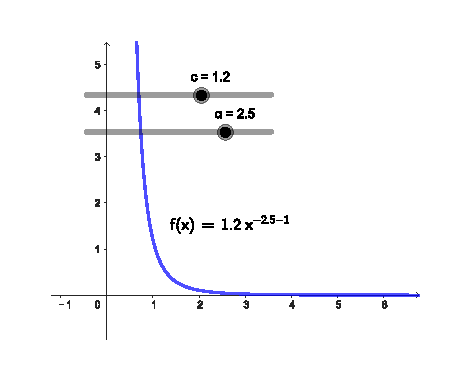
\includegraphics[width=0.5\textwidth]{/0229.pdf} \\

	幂律分布的``互补累积分布函数 F(x)"(CCDF) 是: $\boxed{	P(X \geq x)=cx^{-\alpha}, \quad  x \to \infty }$ \\
	
	注意: CDF 和 CCDF 的区别:  \\
	\begin{tabular}{|p{0.5\textwidth}|p{0.5\textwidth}|}
		\hline
		累积函数 CDF (Cumulative Distribution Function) &   $F_X(x)=P(X\leq x)$\\
		\hline
		互补累计函数 CCDF (Complementary Cumulative Distribution Function) & $F(a)=P(x>a)$. 注意, 这里是大于号(>)! \\
		\hline
	\end{tabular} \\

	
	在统计学中,幂律 power law 表示的是两个量之间的函数关系: 其中一个量的相对变化, 会导致另一个量的相应``幂次比例"的变化,且与初值无关. \\
	
	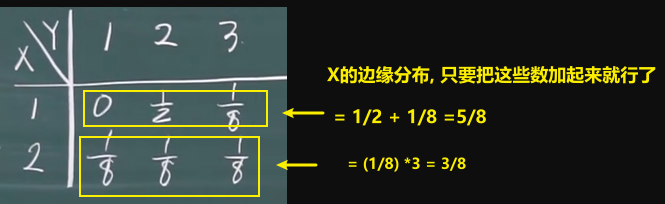
\includegraphics[width=0.6\textwidth]{/0228.png} \\
	
	曲线的横坐标,代表随机变量的取值; 纵坐标,代表发生的概率. \\
	\textbf{幂律分布曲线的含义非常明确 : 在随机变量中,越小的数值, 出现的概率越大; 越大的数值,出现的概率则越小.} 
	
	
	
	\section{性质}
	
	\subsection{尖峰肥尾} 
	
	- 尖峰 : 说明有些x的值很小(赚1000元/月), 但其数量规模大到超乎想象(6亿人). \\
	- 肥尾 : 说明很多极小概率事件(世界首富), 依然有可能发生. \\
	
	如果人的身高, 是符合``幂率分布"的话, 则就会有极少数``身高能长到数公里"的人存在. 
	
	
	
	\subsection{无标度 -- 分形效果}
	
	无标度,也叫``无尺度”, ``尺度无关”. 意思是: 在任何观测尺度下,``幂律分布"都呈现同样的分布特征. 即, 无论你从曲线上截取哪一段, 是长是短, 它都含有二八定律存在(虽然曲率不同). 就相当于``分形"效果. \\	
	一般的分布, 都会有个尺度范围,在这个范围内服从这个分布,超过这个尺度可能就不服从这种分布了。而``幂律分布"没有尺度的限制,不管截取任何一个部分,都仍然呈现幂律分布的特征. \\
	
	比如,图书销量是服从``幂律分布"的 : \\
	- 最畅销那本书的销量, 在前10名销量中占的比例, \\
	- 和前10名的销量, 在前100名的销量中占的比例, \\
	- 和前100名, 在前1000名的总销量中占的比例,\\
	大体都是相同的. 这就是``幂律分布"唯一的数学特征——无标度.
	
	
	
	\subsection{幂律分布让``均值$\mu$"失去意义} 
	
	``正态分布"是一种均匀对称分布, 大多数数据都集中在``均值 $\mu$"附近, 所以均值非常有用, 因为它代表大多数. \\	
	而\textbf{``幂律分布"呢? 它的数据变化幅度非常大,平均值毫无意义.} 比如个人收入,有穷人,也有富豪,把这两群人的资产平均 (人均收入),毫无意义. 
	
	
	
	\subsection{幂律分布中的``波动性(方差$\sigma$)"失去意义}
	幂律分布,随机变量波动的范围非常大,常用的``平均值"、``标准差"到这里都没用了. 
	
	
	\subsection{在``双对数坐标系"下,幂律分布表现为一条斜率为``幂指数的负数"的直线}
	
	自然界中大多数被识别的幂律的指数是这样的:平均值是明确的,但方差不是. 这意味着它们能够出现黑天鹅行为. \\
	
	关于坐标系: \\
	(1) 算术坐标系统(笛卡儿坐标) : 横,纵的刻度, 都是是等距的. \\
	
	(2) ``对数"坐标系统 : \textbf{坐标轴是按照``相等的指数增长变化"表示的.} 举例来说:如果每1cm 代表10的1次方增加,则坐标轴刻度的表示依次为: 1,10,100,1000,10000 ... \\
	
	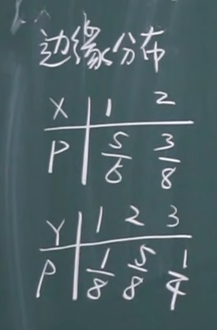
\includegraphics[width=1\textwidth]{/0230.png} \\
	
	\underline{什么时候, 要使用到``对数"坐标系呢?}  \\
	→ 如果所研究的函数的y值, 和自变量x, 在数值上均变化了几个数量级. 比如,已知x和y的数据为:x= 10, 20, 40, 60, 80, 100, 1000, 2000, 3000, 4000  y= 2, 14, 40, 60, 80, 100, 177, 181, 188, 200. 则, 在``直角坐标系"上, 就很难作图. 而换用``对数坐标系", 就能够画出来. \\
	→ \textbf{当需要变换某种``非线性关系"为``线性关系"时.} (比如, ``幂率分布"的概率函数图上.) \\
	
	未完:
	https://baike.baidu.com/item/%E5%8F%8C%E5%AF%B9%E6%95%B0%E5%9D%90%E6%A0%87?fromModule=lemma_search-box
	
	
	(3) ``双对数"坐标: 指两个坐标轴, 都是``对数坐标". 即假如对应于x、y轴,则两轴等刻度情况下,其值``以相应底数, 成次方增长". (注意:在各自坐标轴上的是``真数",不是求对数后的值.) \\

	
	
	
	\subsubsection{真数 : 即 $\boxed{\text{底}^{\text{指}(\text{真数})}=\text{幂}}$中的``指数"}
	什么是``真数 natural(number); antilogarithm"? \\
	即: $
	\underset{\text{底}}{\underbrace{2}}\overset{\text{指,对数}}{\overbrace{^3}}=\overset{\text{幂,真数}}{\overbrace{8}},\ \text{即\ }\log _{\underset{\text{底}}{\underbrace{2}}}\overset{\text{幂,真数}}{\overbrace{8}}=\overset{\text{指,对数}}{\overbrace{3}}
	$ ) \\
	
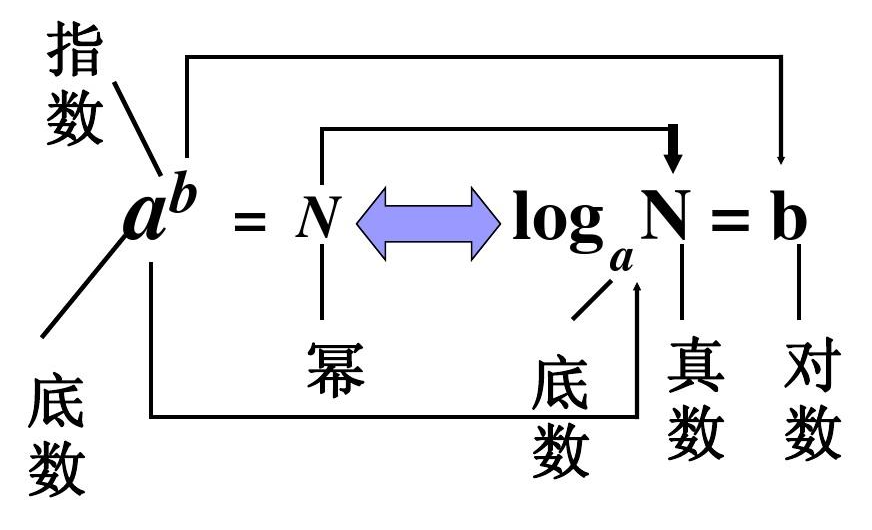
\includegraphics[width=0.35\textwidth]{/0231.png} \\


	
	
	
	
	
	
	
	
	
	
\end{document}